\chapter{Implementation}
\label{ch:implementation}
After the high-level discussion of the programming language and compiler, as well as the formal definitions for both the syntax and translations, in the following chapter, we discuss the concrete implementations of the different stages of the compiler. Firstly, we present the implementation of some general classes and concepts in the compiler as well as the compiler class, which calls and connects all other stages. Next, we discuss the lexical and syntactic analysis of the program code; more specifically, we present the grammar implementation of the language and explain its structure. After the lexical and syntactic analysis, the different parts of the semantic analysis are discussed. Then, the implementation of the code generation and its parts are presented. This is followed by a discussion of the implementation of the optimization. 

\section{Compiler}
\label{sec:implementation_compiler}
% \begin{itemize}
%     \item Static compiler class
%     \begin{itemize}
%         \item General information
%     \end{itemize}
%     \item How are different parts called
%     \item How do they interact?
%     \item Discuss general concepts and classes used by compiler
%     \begin{itemize}
%         \item Compiler data
%         \item IO Handler
%     \end{itemize}
% \end{itemize}
The compiler consists of multiple classes and stages that work together to compile and optimize the given program. While most of the compiler can be divided into discrete stages, there are multiple overarching classes and commonly used structures that do not belong to a certain stage. In the following section, we discuss the implementation of general functionalities and introduce the commonly used structures.

When the compiler program is started, the main function calls the Command Line Interface class to parse the arguments to the compiler data class. The compiler data is used to enable and control the compilation process; it contains all required information such as the path to the input and output files. Furthermore, it specifies which optimizations are to be applied to the compiled program. Lastly, it indicates, whether the compilation process is to be executed verbosely. 

After the compiler data is parsed, the main function passes it to the compile function of the compiler class. This is a static class containing general compilation and printing functionalities as well as corresponding properties. We implement it as a static class so that all parts of the program can easily access its functions and properties. The first property of the compiler is the \texttt{Printer} function; its default value is the native console printing function of C\# but it can be set to any arbitrary function that takes a string as an input and does not return anything. While this property is not changed in a normal compilation process, it is used to check the console output of the compiler in the test cases. Secondly, the verbose property indicates whether the compiler prints not only the errors to the user but also the warnings and informational logs.

To interact with the printer property of the compiler, there are a variety of different printing and logging functions; in the end, all use a sing print function that uses the printer property to display a given message. While the printing functions, used for printing errors and warnings, call the print function directly, the logging functions have an additional check so that they only print, if the compiler is executed verbosely. Lastly, the logging functions also use compiler services of the runtime to allow for special injections. All of the logging functions have the optional member name and line number arguments that are annotated with special attribute. In turn, if the optional arguments are not set, the compiler injects the name of the caller for this function as well as the line number where it was called. This can be helpful when trying to debug issues with the compiler.  

The compile function handles the entire remaining compilation process. First, it retrieves the program code from the given input path. For the reading and saving of files, a separate \texttt{IOHandler} class exists that has some basic logic for reading and writing files. Then, the parse tree is created and passed to the semantic analysis of the compiler. Here all errors and warning are printed to the used. If any errors are thrown, the compilation is aborted. Next, the code is generated from the parse tree. If the compilation resulted in error, again, the compilation is arbored. After the code is generated, it is optimized based on the optimizations given in the compiler data. Lastly, the resulting program is written to the file specified by the output path.

\subsection{Command Line Interface}
\label{sec:implementation_cli}
As the interface between the programmer and the compiler itself, the command line interface (CLI) is an essential part of the compiler. 
Its purpose is to interact with the programmer and created the compiler data which specifies the behavior of the compiler. 
To achieve this, the CLI consists of two different parts. The first are the attributes that are used to annotate the compiler data class and the second part is the CLI Handler; it parses the input arguments and creates the compiler data from them. Additionally, it print the help text to the console if needed.

An attribute is a C\# class that can be used to annotate fields and properties of another class; together with reflection, it can be used to create a modular and easily extendable compiler data class with parameters and descriptions for each compiler data property. Reflection allows programs to get information on types of loaded assemblies. In our case, we are interested in the information on classes, more specifically information on properties of the compiler data class. We create custom attributes with a class that inherits from the \texttt{Attribute} class and contains the required information about the properties we need. With reflection, our program can get a list of all properties with specific attributes and use their information to create, \eg, the help text of the CLI. In turn, we have two custom attributes in our program. The first it the \texttt{CLIParameterAttribute} which specifies both the short and long name of an attribute corresponding to the compiler data property. For example, in the case of the input path property, the short name is a lower case ``i'' and the long name is ``input''. The second attribute is the \texttt{CLIDescriptionAttribute}; it contains a description for the property it is applied to. Then, this description can be display in the help text. In the case of the input path property, the description describes that the parameter describes the path to the input file. The code for the input path property example is depicted in Fig.~\ref{fig:implementation_inputPathAttribute}.

\begin{figure}[htp]
    \centering
    \begin{lstlisting}[language=csh]
[CLIParameter('i', "input")]
[CLIDescription("Path to the input file.")]
public string InputPath { get; set; } = string.Empty;
    \end{lstlisting}
    \caption{The input path property declaration with its parameter and description attribute.}
    \label{fig:implementation_inputPathAttribute}
\end{figure}

To parse the command line arguments and create the compiler data from it, the command line interface class is used; it consists of functions to parse the arguments and print the help text to the console. Since the syntax for the CLI argument input is very basic, the command line parsing itself is basic. The input string is split at each space and given to the function as a string array. First, the function retrieves the CLI parameter attributes for all compiler data properties. Then, it iterates over the string array and, for each array entry, checks whether the parameter attribute matches the string; for example, in the case of the input path property, the string would have to be either ``-i'' or ``--input''. If this is the case, the corresponding parsing function, depending on the matched argument, is called with the string array and a reference to current index. A reference to the index is used to allow for further changes to the index, depending on the number of possible arguments for a parameter. For example, the verbose parameter will always return true and not change the index while a path parameter will increment the index and return the next string of the array. If no attribute can be matched or an argument exception is thrown in the process, the compiler will notify the user of the invalid or missing argument and print the help text to clarify the compiler options.

The help text is created based on the attributes of the properties in the compiler data class. Firstly, the function retrieves both the parameter and description attributes. Since the compiler data class does not include the help parameter, as it is only used in the CLI context, the help text manually prints its information. Then, the parameters are iterated. For each parameter, a matching description is searched. If no description can be found, the text defaults to a message indicating that non is available. Lastly, both the parameter and corresponding description are printed to the console.

\subsection{Symbols}
\label{sec:implementation_symbols}
One part that is used in most stages of the compilation process, mainly the semantic analysis and code generation, are the symbols; they are used to store all necessary information on data type, composite gates, and similar object in the language. The basis is an abstract symbol class that consists of an identifier and error context property. The identifier uniquely identifies a symbol in the scope it is used while the error context saves information about the symbol and its declaration environment to be used for possible error messages. In total there are eight different symbols that are derived from the class. In the following, we discuss these symbols and how they are used in the compiler. The hierarchy of the symbol classes is depicted in an UML diagram in Fig.~\ref{fig:implementation_uml_symbols}.

\begin{figure}[htp]
    \centering
    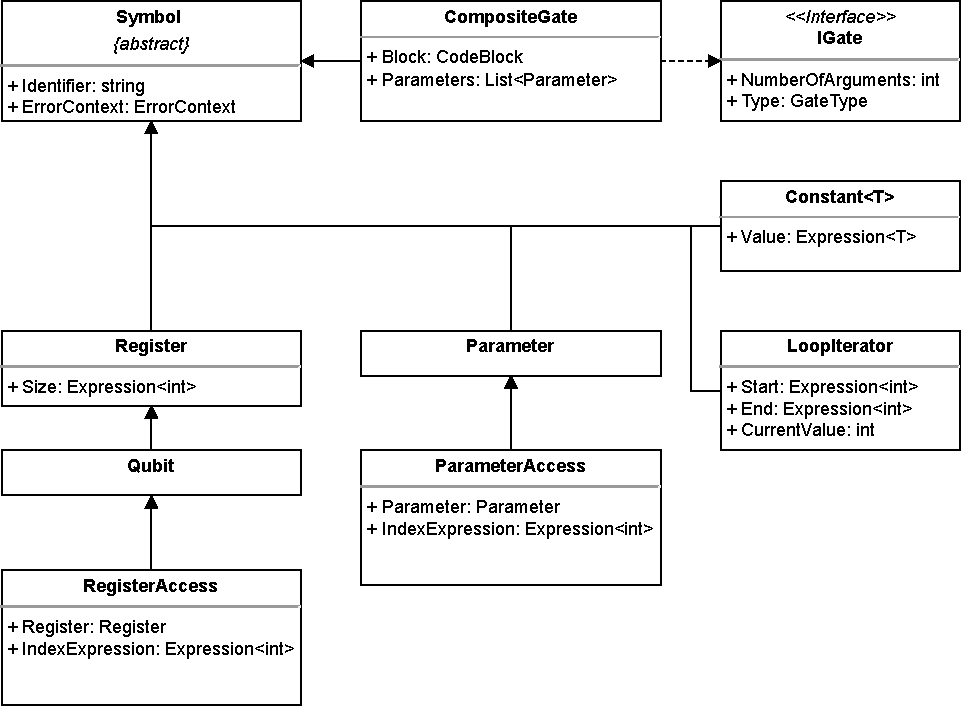
\includegraphics[width=.9\textwidth]{../figures/uml_symbols.pdf}
    \caption{UML diagram of the different symbols.}
    \label{fig:implementation_uml_symbols}
\end{figure}

There are three different symbol for quantum data types. The first kind is the register. Futhermore, it is the basis of all other quantum data type symbols. Besides the inherited properties, it consists of an expression that represents the size of the register. The expression specifying the size of the register may not be evaluable when its symbols is crease because the value of some identifiers may be known only at generation time.\todo{Introduce ``generation time'' as phrase with clear meaning}
For example, the body of a loop statement is unrolled at generation time and the values of the loop iterator depends on this iteration. In turn, the value of the iterator identifier may not be known when the register symbol is created. Therefore, instead of saving a constant value, the symbol specifies the expression for its size. Then, when the code is generated and all values are know, the expression can be evaluated.    

Next, the qubit symbol inherits from the register. While physically the qubit is the basic element and a register consist of qubits, in our case, it is useful to assume that a qubit is a special case of a register where the size is one so that the qubit can inherit the register symbol properties and functions. Furthermore, instead of differentiating between a qubit and register declaration, a register declaration is sufficient for this hierarchy, only requiring a differentiation when printing the code. In turn, all registers with size one are inherently optimized to be qubit in the target code. Besides setting the size to one, the qubit symbol has no additional attributes.

The last quantum data type symbol is the register access. This symbol is necessary because the access of a register is not implemented as an expression. Since a register access cannot be used in any expression and only in the context of a gate application or if-statement, instead of implementing special quantum expressions, that can only be used in limited cases, we create another symbol. The register access symbol inherit from the qubit symbol as it can be used whenever a qubit symbol can be used. For example, in the case of a gate application statement, a list of qubits, to which the gate is applied, is saved. In turn, since each register access is a qubit, no additional list or differentiation is required for the gate application, only a virtual function to return the translated qubit code. The symbol also contains an integer expression that specified which index is accessed and the register which is accessed. Similar to the size expression of the register symbol, the expression is saved since it may not be evaluable when the symbol is created.

There are two symbol for classical data; these are the constant symbol and the loop iterator. The constant symbol represents a constant variable of differing types. To allow for different variable types, the symbol has a generic parameter \texttt{T}. Additionally, the generic parameter is restricted to implementing the number interface, indicating that it is a numeric type. Furthermore, as with the other symbols where a property may depend on a value that is not know at the time of creation, the constant symbol value is given by an expression. This expression is of the type \texttt{T}.

Secondly, the loop iterator symbol is the other symbol used to represent classical data; however, it is specifically designed for the loop statement of our language and its special properties. It is used to unroll the loop body and propagate the value of the current iteration of the loop. To achieve this, the symbol contains the start and end indices as integer expression; they can be evaluated when the code is being generated. Furthermore, the symbol contains a current value property which contains the value of the current iteration. When the code for the loop body is unrolled by being iterated, any reference to the iterator symbol will evaluate to the current value.  

The last three symbol are all related to the composite gates. Firstly, there is the composite gate symbol itself. It is created when a composite gate is declared and, later on, is used whenever it is referenced in a gate application statement. To allow for predefined gate, an interface is declared that represent the important attributes of a gate; these are the number of arguments to the gate and the gate type. The gate type differentiates between the different predefined gate such as the Hadamard or $X$ gate and the composite gates. This gate interface is implemented by the composite gate. Besides the properties required by the gate interface, the composite gate symbol consists of a block property and parameter property. The block property contains the code block that is the body of the composite gate; it is used to inline to statements of the gate whenever it is applied. Secondly, the parameters are a list of parameter symbols that represent the arguments that can be passed to the composite gate.   

The second kind of composite gate related symbols are parameter and parameter access symbols. Both represent an argument to a composite gate and serve as a placeholder for the symbol of the argument that if passed when the gate is applied. When inlining, the placeholder, \ie the parameter symbol, is mapped to the given argument. Furthermore, while the composite gates themselves can only operate on the previously discuss quantum data type symbols, the programmer does not specify the type of the argument, which can be both a qubit or quantum register, when declaring the composite gate. Therefore, we introduce a symbol which will ignore type checking until the composite gate is called and the arguments are specified. Then, if an argument is of an invalid type for a specific use, a type error is thrown. Similar to the register access, an additional parameter access symbol is required because an access cannot be represented as an expression; it inherits from the parameter symbol, has a reference to the parameter that is access and an integer expression that evaluates to the access index at generation time.

\subsection{Symbol Table}
\label{sec:implementation_symbolTable}
The symbol table is a data structure that saves all symbol information and offers function for adding new symbols and retrieving symbol information. For example, a new symbol can be added with the \texttt{AddSymbol} function and symbol information can be obtained based on the identifier with with \texttt{GetSymbolInfo} function.

To allow for different symbol contexts, the scope data structure is used. Scopes are used enable the declaration of different variables with the same identifier in independent scopes, \ie two scope where neither is the others ancestor nor descendent. The scope class contains an identifier dictionary that maps a string, in this case representing the identifier, to the corresponding symbol. Because of the quantum if-statement, a scope can also be guarded by a qubit. Therefore, a scope has an optional guard symbol that either references the symbol that guards the scope, and all descendants, or is null. Lastly, the scope contains a reference to the code block it belongs to. While the parse tree is traversed, each statement is added to the code block of the current scope. Later, the code block can be passed along in the generation to, \eg, create the loop statement belonging to the scope. 

The scopes are saved in the symbol on a stack. Each time a new code block is entered when traversing the parse tree, a new scope if pushed onto the scope stack. Similarly, each time a block is exited, the scope stack is popped to remove the latest scope from the data structure. To simplify the interactions with the scope stack, the symbol table contains both a current scope and current identifier map property; both reference the top-most scope on the stack and the identifier map of the current scope respectively.

While the scope data structure holds a reference to a reference to the guard symbol, the symbol is know before the creation of the current scope because first the if-statement is traversed then the code block. Therefore, the class interacting with the symbol table would need to save the current identifier and pass it to the push scope function. To avoid this additional complexity, the symbol table hold a guard stack that can be interacted with by using the additional \texttt{PushGuard} and \texttt{PopGuard} functions. In turn, the symbol table can use the scope stack to pass the current guard to an newly created scope. Additionally, guards and scopes abstracted when using the symbol table such that the class traversing the parse tree only needs to push and pop the correct information and is not required to save the current guard information. 

Lastly, the symbol table contains a property that generate a unique identifier. To achieve this, it contains a private integer field \texttt{\_uniqueId} that is initialized with a value of zero. Each time the unique identifier property is retrieved, the id is incremented. The identifier is just the id with a ``id\_'' prefix. The property is used when generating the OpenQASM code as it does not allow for different variables with the same identifier. While this is a very simplistic approach, this resulting identifiers are always unique, as long as the same symbol table is used, and the resulting identifiers are predictable. This predictability is especially helpful when creating test cases for the translation of source code as we can simply give the expected target code. 

\section{Lexical and syntactic analysis}
\label{sec:implementation_syntaxAnalysis}
The lexical and syntactic analysis steps of the compiler are not implemented by hand but ANTLR4 is used to generate both the lexer and parser. In Sec.~\ref{sec:background_compilerTools}, a short introduction is given into the generation tool. The tool does not only generate the lexer and parser for the language but also some data structures, like the parse tree, and abstract classes that are used for the following compiler steps. In the following, we discuss the ANTLR grammar of Luie and give an overview of the different classes that are generated by ANTLR.

\subsection{Grammar}
\label{sec:implementation_grammar}
The entry point for the grammar is a parsing rule called \texttt{parse}. It states that the program consists of a main code block followed by the end of file lexer token \texttt{EOF}. The main code block starts with arbitrarily many gate declarations, or none at all, and is followed by any number of declarations and statements in any order, or none at all. Similarly, a ``normal'' code block also consists of any number of declarations and statement; however, it does not allow for gate declaration. The grammar for the entry point, main and general code block is depicted in Fig.~\ref{fig:implementation_grammarStructure}

\begin{figure}[htp]
    \centering
    \lstinputlisting[style=ANTLR]{../figures/code/grammar_structure.g4}
    \caption{The basic structure parsing rules of Luie.}
    \label{fig:implementation_grammarStructure}
\end{figure}

While syntactically it would be equal to say the main block consists of gate declarations and a code block, the code generation implementation requires the main code block to directly hold the declarations and statements. Internally, each code block object holds a list of declarations and statements which, in turn, can hold references to other codeblocks. However, a block itself cannot hold a reference to another block. Furthermore, the code generation is only called on the main code block which, then, recursively calls the code generation for each declaration and statement. Therefore, the main code block needs to contain the declarations and statements directly, otherwise the code generation will alway generate an empty program. 

There are three kinds of declaration rules in the grammar. The first is the declaration rule for qubits and registers. It start with the register keyword lexer token, followed by an optional expression in brackets giving the size. If no size is given, a qubit is created; otherwise, a register with the given size is created. The identifier for the qubit or register is the last part of the rule. 

\begin{figure}[htp]
    \centering
    \lstinputlisting[style=ANTLR]{../figures/code/grammar_declarations.g4}
    \caption{The parsing rules for declarations in Luie.}
    \label{fig:implementation_grammarDeclarations}
\end{figure}

Next, the constant declaration rule is used to declare constants that can be used at compile time, \eg for the size of registers or to given the number of loop iterations. Similar to register and qubit declarations rule, the rule start with a constant keyword token. Then, the identifier is given and separated from the type of the constant with a colon. Lastly the expression for the value of the constant is given after an equality sign.

The final declaration rule is used for composite gate. Again, it starts with a corresponding keyword and is followed by the identifier of the gate. Next, the optional\todo{Should gate parameters be optional?} gate parameter rule is given in parenthesis. The gate parameter rule matches any number of identifiers, separated by commas, requiring at least one identifier. Lastly, the gate declaration rule ends with a code block rule. 

All declaration rules are given in Fig.\ref{fig:implementation_grammarDeclarations}. Note that the depicted grammar is semantically equal to the grammar used in the implementation; however, some of the formatting and naming was adjusted for the thesis.
\unsure{should this be specifically stated?}

The grammar contains four different type of statements. The first is the gate applications statements, followed by two the control flow statement and, lastly, the skip statement. The gate application statement start with the gate rule. A gate can either be a constant, or predefined, gate such as the Hadamard or $X$ gate, a parameterized gate, such as $P(\lambda)$, or a composite gate given by its identifier. In the case of the parameterized gate, the parameter is given by an expression. Following the gate rule, the register rules specify to which qubits or registers the gate is applied. Here, at least one argument is required but there can be arbitrarily many arguments, each separated by a comma. A register or qubit can either be given by the corresponding identifier or as a register access. In this case, the index to be accessed is given by an expression. The grammar rules related to the gate application statement are also depicted in Fig.~\ref{fig:implementation_grammarGateStatements}. 

\begin{figure}[]
    \centering
    \lstinputlisting[style=ANTLR]{../figures/code/grammar_gateStatements.g4}
    \caption{The parsing rules for gate statements in Luie.}
    \label{fig:implementation_grammarGateStatements}
\end{figure}

Next, the first control flow statement is the if statement. It starts with the \texttt{if} keyword which is followed by the register rule. This register is the qubit which controls the execution of the body. After the control bit is specified, the \texttt{ifStat} rule gives the code block which is controlled by the control bit. This is followed by an optional else block; it start with the \texttt{else} keyword and the corresponding code block. Both the main and else code blocks are introduced by the \texttt{do} keyword. Lastly, the if statement is ended with the \texttt{end} keyword.

\begin{figure}[b]
    \centering
    \lstinputlisting[style=ANTLR]{../figures/code/grammar_controlflowStatements.g4}
    \caption{The parsing rules for the control flow statements in Luie.}
    \label{fig:implementation_controlFlowStatements}
\end{figure}

The second and lst control flow statement is the loop statement. Similar to other statements and declarations, it starts with the corresponding \texttt{for} keyword. Next, the identifier for the loop iterator is given, followed by the \texttt{in} keyword. Then, the range for the loop statement is specified. There are three different possibilities to give the range. Firstly, the simplest syntax for a range is the start and end indices separated by two dots. The other two options both start with the \texttt{range} keyword followed by arguments in parenthesis. The first option only gives the length of the range as an expression while the second specifies both the start and end indices as expressions. Lastly, the body of the loop is a code block surrounded by the \texttt{do} and \texttt{end} keywords.   
The grammar rules for both control flow statements is depicted in Fig.~\ref{fig:implementation_controlFlowStatements}.

An expression mainly consists of three different different grammar rule. The first rule is the expression rule itself. It matches the operands with the lowest precedence. In our case, these are both the addition and subtraction operation. The left-hand side of the addition and subtraction is also a expression. In contrast, the right-hand side specifies a term rule. Alternatively, the expression can also be neither an addition nor subtraction but just a term. 

Similar to the expression rule, the term represents two operations. In this case, they are the multiplication and division operations with neither the hightest nor lowest precedence. While the left-hand side of both operations matches the term rule again, the right-hand side specifies a factor. Again, the term can also be neither a multiplication nor division but a factor instead.

\begin{figure}[htp]
    \centering
    \lstinputlisting[style=ANTLR]{../figures/code/grammar_expression.g4}
    \caption{The parsing rules for an expression in Luie.}
    \label{fig:implementation_expression}
\end{figure}

Lastly, the factor rule includes all operations with the highest precedence. The first option is an expression is parenthesis. 
The second possibility is a negate factor. Finally, the factor can either be the result of a function, the value of an identifier, or an integer value itself. While the value of an identifier is just given by the identifier itself and the integer value is specified by giving the integer, the result of a function is given by the function rule. The function rule starts with the name of the function. An example of a function name is \texttt{sizeof} or \texttt{power}. The name of the function is followed by the function parameters in parenthesis. The function parameters are either a list of identifiers or expressions separated by commas. Both require at least one identifier of expression but allow of arbitrarily many. 
% While expressions also allow for identifiers,
\change{expression can also by only identifiers -> can likly lead to errors -> \emph{\color{red} fix code}}
All expression grammar rules as well as the function related rules are given in Fig.~\ref{fig:implementation_expression}. Furthermore, all terminal symbols such as, \eg, the different functions and the regular expressions for identifiers and integers are given in Sec.~\ref{appendix:grammar_terminals} of the appendix.

\subsection{Data structures and classes}
\label{sec:implementation_syntax_dataStructuresClasses}
Based on the grammar, discussed in the previous section, the ANTLR tool generates different classes and files that can be used for the lexical and syntactic analysis of the source program. The tool generates token files as well as the necessary classes for the analyses; these classes inherit from abstract bases classes such as \texttt{Lexer} or \texttt{Parser} that are contained in the ANTLR runtime package. Additionally, the tool can also generate optional classes that can be used for the semantic analysis of the program or for code generation; these classes are the \texttt{Listener} and \texttt{Visitor}.

After the lexical and syntactic analysis yield the parse tree of the source code, both the listener and visitor classes can be used to traverse the tree. They implement a list of virtual functions without any effect. Then, these can be overridden and extended by custom functionality. The visitor class has a generic type parameter \texttt{Result} and implement a visit function that returns \texttt{Result} for each grammar rule. For example, in the case of our grammar, as discussed in Sec.~\ref{sec:implementation_grammar}, the visitor class implements, among other things, a \texttt{VisitParse} and \texttt{VisitMainblock} function. Additionally, for each grammar rule there exists a context which provides information about the rule such as its the line and column in the source code. Furthermore, the context can be used to get information about the terminal in a rule. For example, in the case of the expression rule, the context can be used to learn which operation, either addition or subtraction, was given. The parse tree can be traversed by implementing the different visit functions and, in their implementation, having them call their child rules.

In contrast, the listener class does not have a generic type parameter and, in turn, its functions do not return anything either. However, instead of implementing a visit function for each grammar rule, the listener implements both a enter and exit function for each rule. Furthermore, the functions corresponding to the children in the parse tree are not explicitly but the tree is traversed by a walker class and the enter and exit functions are called in order of the traversal. Therefore, the \texttt{EnterParse} function is the first function that will be called, while \texttt{ExitParse} is the last. Similar to the visitor functions, both the enter and exit functions have the context of the corresponding grammar rule as an argument. Both our semantic analysis and code generation implementation create custom listener classes instead of visitors.\todo{Why use listeners instead of visitors?}


\section{Semantic Analysis}
\label{sec:implementation_semenaticAnalayis}
The second step in our compilation process is the semantic analysis of the input program. The analysis checks for any semantic errors in the code that can be detected before the next compilation step, the code generation. Our implementation of the semantic analysis differentiates between a declaration analysis and type checking. The declaration analysis is concerned with checking for errors related to the declaration of variables. For example, when a variable is used, it check whether it was declared previously or, when a variable is declared, the analysis ensure that the identifier is not in use in the current scope. In contrast, the type checking ensures that the type of a variable is consistent with the use of the variable. 

Both analyses are implemented as separate \texttt{Listeners}.
\todo{describe in \ref{sec:implementation_syntax_dataStructuresClasses}} 
This is done to separate both classes and give them concrete purposes while making the overall structure of the compiler more modular. In turn, since both analyses are implemented separately, they currently each require a traversal of the parse tree making the semantic analysis more inefficient. However, this can easily be addressed by writing a \texttt{Listener} that wraps both analyses, traverses the parse tree only once, and calls the corresponding function for each wrapped analysis.     

\subsection{Declaration Analysis}
\label{sec:implementation_declarationAnalayis}
The declaration analysis reports any errors that caused by the use of identifiers in invalid contexts; these are the use of an undeclared variable, the declaration of a variable in a context where it is already defined, and the use of a qubit in a code block which is guarded by itself.
\todo{Define when a code block is guarded by a qubit.}
Additionally, it also reports a warning when a variable is declared but never used.

For its analysis, the class creates a symbol table and adds any symbol that is declared. Further, is executes all other functions required for a valid analysis with the symbol table, like pushing scopes onto and popping them from the stack in the symbol table at the locations in the parse tree transversal where it is required. Before adding a symbol to the table, \ie every time the parse tree transversal exits a declaration, the \texttt{Listener} checks whether the identifier is already declared in the current context; if this is the case, the corresponding error is reported. Similarly, each time an identifier is referenced outside of a declaration, the analysis ensures that the variable is defined, otherwise it reports the corresponding error as well. Lastly, whenever a register rule is encountered in the transversal, the analysis not only checks that the variable is declared but also whether the current code block is guarded by the referenced register. If this is the case, the analysis reports an error. While the register parsing rule is only used for gate applications and if-statements and not for function calls such as \texttt{sizeof}, only performing the check the register rule cannot result in an invalid use of an identifier. This is the case because all function calls result in constant values and only refer to properties of a register, not the register itself; therefore, the compiled program will not have a reference to the register in the controlled context.\todo{Cannot check for all cases, some need to be at generation time}

While the symbol table suffices for reporting the previous errors, it does not track the usage of symbols. Therefore, it cannot be used for the unused symbol warning. For this analysis, the class contains a dictionary that maps a symbol to the number of references. Each time a symbol is added to the symbol table, the corresponding entry in the dictionary is initialized to zero. Then, for every reference to the symbol, its usage counter is incremented. At the end of the tree transversal, specifically when exiting the main code block, the analysis iterates over all entries in the dictionary and reports a warning whenever the usage counter is still $0$. However, there is an exception if an identifier is the underscore character so that it can be used as a throwaway variable, similar to other programming language.  

\subsection{Type Checking}
\label{sec:implementation_typeCheckingAnalayis}
\begin{itemize}
    \item What does type checking do?
    \begin{itemize}
        \item checks the use of symbols
        \item ensure that they are used in a valid context
    \end{itemize}
    \item How is this accomplished?
    \begin{itemize}
        \item for each use of an identifier, the type of the symbol is checked
        \item Register only allows either register, and if index is given, cannot be qubit, any parameter type checking is skipped
        \item Identifier in factor rule can only either be loop iterator or constant symbol, because numeric value is required, in turn, eg register is not valid
        \item for gate application, all given registers are checked, is not register type error, composite gates allow registers, constant gates only qubits
        \item furthermore, number of arguments is checked against required
        \item if statement requires qubit or register with qubit access
        \item range is checked for valid range, can throw invalid range exception
        \item when leaving the gate rule, and an identifier is given, corresponding symbol needs to be a composite gate
        \item function allows for identifiers when using size of function, only allows registers
        \item 
    \end{itemize}
    \item Similar to declaration analysis, symbol table is used
    \item All declarations correctly add the symbols so that the info can be used to for the type checking, additionally the scopes are pushed  
\end{itemize}
Type checking is used to ensure that any use of a symbol occurs in a valid context for this symbol. For example, while a qubit symbol can be used as the argument for a gate application, it does not represent a classical numerical value and, therefore, cannot be used in the context of a factor. Similar to the declaration analysis, a symbol table is used and all symbols, that are declared while traversing the tree, are added to it. Additionally, the scopes are also pushed and popped according to the traversal to allow differently typed variables in independent scopes.

To check the use of a symbol, each grammar rule where an identifier can be used checks its type. To do this, each function gets the identifier string and retrieves the corresponding symbol information from the symbol table. In the case of the register rule, only register symbols are allowed. The 

\subsection{Error Handling}
\label{sec:implementation_semanticAnalayis_errorHandling}
Error handling is an essential part of both the semantic analysis and code generation phase of the compiler; without clear and informative error messages, debugging compilation error is both challenging and tedious. Therefore, our compiler contains a number of different compilation errors. All there errors inherit from an abstract compilation error class. 

The abstract compilation error class contains three different properties. The first property is the error type. Currently, there are two different error type possible in the compiler, a warning and a critical error. While a warning indicates an issue with the source program which can still be compiler, a critical error in the source code cannot be compiled and results in the abortion of the compilation progress. Secondly, the description property should hold a description of the error that can be used to inform the programmer what issue occurred. Lastly, the error context saves relevant information about the source code properties of the error; it is implemented as a \texttt{struct} that contains both the line and column index of the source code location of the error. The error context can be created either from the line and column directly, the token where the error occurred, or the parsing rule with which the error is associated. In many cases, the error context can be created when the error occurs. For example, if an undefined identifier error is found in the declaration analysis, the parser rule context is given an the error can easily be created from it. However, in other cases, error may be thrown at generation time and the corresponding parser rule context may no longer be know. Therefore, all symbol also contain the error context corresponding to their declaration. 

While the abstract compilation error class contains general properties that are required for all errors, each error may contain additional properties that are required to give a clear and informative description of the error. Since many error occur in reference to a specific identifiers, the compiler uses an additional abstract identifier error that contains a string property which holds the identifier. The invalid access, type, invalid size, redefine, and use of guard error are all identifier errors. While the undefined error is also related to an identifier, it holds a list of identifiers instead of just a single one. This is because it is also used for undefined identifiers in an expression, where multiple are possible. Since they are in the same context, \ie the same expression, they are accumulated into a single error to reduce the number of errors. Additionally, many error are related to an invalid argument or invalid number of arguments. In this case, the given argument or number of arguments is saved in the error object; this is the case for the invalid function arguments, invalid number of argument, invalid access, invalid range, and invalid size error. In some cases, the required arguments are apparent from other properties, \eg the invalid number of arguments error contains a gate interface which specifies the number of required arguments. In contrast, other error specifically contains the required number of arguments, as they are specified by other properties, \eg the invalid function argument. All the different errors, including their respective properties, are depicted in Fig.~\ref{fig:implementation_uml_errors}.

\begin{figure}[htp]
    \centering
    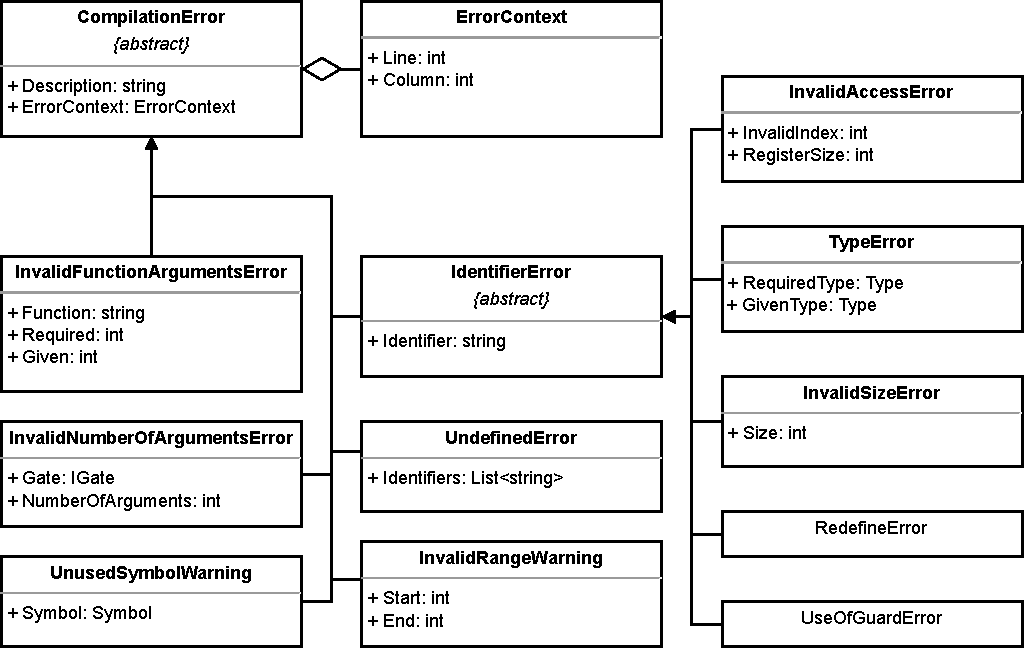
\includegraphics[width=.9\textwidth]{../figures/uml_errors.pdf}
    \caption{UML diagram of the different errors.}
    \label{fig:implementation_uml_errors}
\end{figure}

One advantage of a semantic analysis separate from the code generation is that, if an error is found, the semantic analysis can continue. For example, if an undefined identifier error occurs while generating code, the code generation can no longer continue as the identifier cannot be mapped to a symbol and, therefore, the information for the code generation is incomplete. However, a semantic analysis can continue as it does not need any more information about a symbol than its existence. In turn, while error in the code generation phase use typical error handling with exceptions that abort the tree traversal, the semantic analysis uses a custom error handler. Mainly, this error handler object consists of a list of compilation error and a report function that takes an error and adds it to the list. Additionally, the handler also contains properties that indicate whether it contains critical errors and two lists that return only the critical errors or warnings respectively. After the semantic analysis, the compiler will iterate over the errors in the handler in print them as either errors or warnings, depending on their error type.\unsure{Internal exceptions explained here?}

\section{Code Generation}
\label{sec:implementation_codeGen}
To generate the target code, first, the parse tree is traverse and the source code is translated to an in-memory representation consisting of objects corresponding to different language concept. These concepts can be divided into three different kinds, statements, declarations, and code blocks. All of the objects implement an interface; it requires a translation function that translates the source code representation to the target code representation. The target code representation is a collection of objects that describe an OpenQASM program; they can be translated directly to the textual OpenQASM code. In the following, we discuss the generation of the source code representation from the parse tree, the translation from the source code to the target code representation, and any other utilities that are used in the process.

\subsection{Source Code Representation}
\label{sec:implementation_sourceCode}
Similar to the implementation of the semantic analysis, the parse tree is traversed with another custom listener. However, in contrast to the semantic analysis, the code generation listener does not directly interact with a symbol table but uses a separate code generation handler.

The code generation handler facilitates the creation of the source code representation when traversing the parse tree. Firstly, it contains a main code block; this code block is initiated as an empty code block without a parent when the handler is created. Furthermore, it will hold, directly or indirectly, the references to all other source code objects. The second important property is the symbol table. The handler implements different methods for interaction with this table. For example, it contains methods for both pushing and popping scopes as well as guards. Additionally, the handler implants unique functions for each symbol that can be added to the table, with a protected general function. This is done because some symbols need additional logic when they are added to the symbol table. For example, when a register symbol is added to the table, a register declarations is also added to the current code block.

\subsection{Translation}
\label{sec:implementation_translation}

\subsection{Target Code Representation}
\label{sec:implementation_targetCode}



\section{Optimization}
\label{sec:eval_optimization}
The optimizations, which are applied to the quantum circuit, are the first aspect we want to evaluate. For this, we apply our optimizations to variants of the same algorithm, the quantum ripple-carry adder. Firstly, we analyze the optimizations to the adder when given classical inputs. Next, we evaluate the optimizations of the adder for inputs in superposition with different register sizes. Lastly, we compare our optimizations to optimizations that are applied by the default Qiskit transpilation process of quantum circuits.

In our first example, we use the inputs $a = \ket{1}$ and $b = \ket{15}$, with both the input and output carry qubit having a value of $\ket{0}$. Furthermore, both input registers have a size of four qubits and, in turn, have $2^4 = 16$ possible classical values. After the adder is applied, the $a$ register and carry input, per definition, remain at their initial values of $\ket{1}$ and $\ket{0}$, respectively. In contrast, the $b$ register now has a value of $\ket{0}$ and the carry output a value of $\ket{1}$, indicating that the result of the addition is $\ket{16}$.
The quantum circuit corresponding to the example before optimization rules are applied is depicted in Fig.~\ref{fig:eval_adder_circuit}.
\begin{figure}[htp]
    \centering     
    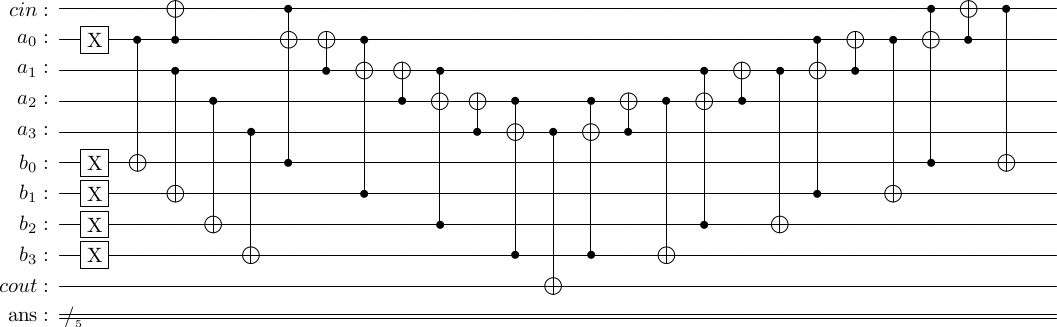
\includegraphics[width=\textwidth]{../figures/images/adderCircuit.png}
    \caption{An unoptimized circuit of a quantum ripple-carry adder.}
    \label{fig:eval_adder_circuit}
\end{figure}

Since the circuit only consists of $X$, controlled-not, and Toffoli gates, neither the Hadamard reductions nor control reversal optimization rules can be applied to the circuit. However, both the peeping control and null gate optimizations can be applied. Whenever a qubit wire contains a known value of $\ket{0}$, the controlled gates can be removed. For the opposite case, the control can be removed and the resulting $X$ gate can be removed when in combination with another $X$ gate. In turn, the circuit can be optimized such that the resulting one only contains gates that initialize the result; only two $X$ gates remain. While the first gate flips the first qubit of the $a$ register, initializing it to $\ket{1}$, the second flips the carry output qubit, indicating a result of $\ket{16}$. The OpenQASM code for the optimized circuit is depicted in App.~\ref{appendix:classicalInputs_optimized}.

In the second example, we input a value in superposition. Now, register $a$ contains a value of $\frac{1}{\sqrt{2}} (\ket{0} + \ket{3})$ and register $b$ contains a value of $\ket{4}$. Again, both carry qubits are initialized to $\ket{0}$. After the adder gate is applied, the carry qubits and register $a$ remain as initialized. However, the $b$ register now has a value of $\frac{1}{\sqrt{2}} (\ket{4} + \ket{7})$.
Since the input is now no longer a classical value, the peeping control optimization can only be applied in a few cases. In turn, only twelve gates are removed. The optimized quantum program is depicted in App.~\ref{appendix:superposInputs_optimized}. In other cases, even fewer optimizations are applied; \eg, with an input of $b = \ket{15}$, only four gates are removed while four Toffoli gates are optimized to controlled-not gates.
While the optimizations are not as effective for inputs in superposition, they can optimize significant parts of the program. For example, when we repeat both examples but increase the size of the registers to $64$ qubits, the optimized circuit contains the same amount of gates. In these cases, if qubits are not entangled by the data in superposition, all gate applications to their wires, except for the initializations, can be removed.

We also compared the optimizations applied by our compiler to the default optimizations that are applied by the Qiskit transpilation process. Qiskit\footnote{\url{https://github.com/Qiskit/qiskit/}}~\cite{JTK*24} is a software development kit for building, simulating, and transpiling quantum circuits. Additionally, the kit can interpret OpenQASM programs and build quantum circuits from them. When transpiling quantum circuits with Qiskit, \ie, transforming to a specific domain such as another basis gate set, the kit can perform optimizations to the circuit based on an optimization level. For the comparison, we used the quantum ripple-carry adder implementation provided by the OpenQASM repository\footnote{\url{https://github.com/openqasm/openqasm/blob/main/examples/adder.qasm}}. The code for the program is depicted in Fig.~\ref{fig:eval_adder_qasm}. The program can then be loaded with Qiskit and built into a quantum circuit. To apply the default optimizations of Qiskit, we transpile the circuit with the highest optimization level to the base gate set our compiler translates to, \ie, $\{X, Y, Z, CX, CCX, H\}$. While our compiler translates to arbitrary controlled gates, they are not used in this example. Furthermore, even the $Y$, $Z$, and Hadamard gates are redundant as they are not used.

\begin{figure}[htp]
    \centering     
    \lstinputlisting[style=QASM]{../figures/code/evaluation/adder.qasm}
    \caption{An OpenQASM 3 implementation of a quantum ripple-carry adder circuit.}
    \label{fig:eval_adder_qasm}
\end{figure}

However, while the Qiskit transpilation can apply many optimizations such as null gate optimizations, the default rule set does not contain a rule similar to our peeping control optimization rule. In turn, no controlled gates can be optimized in the circuit. Furthermore, since the null gate optimizations can only be applied after peeping control rules were applied, the transpilation process does not apply any optimizations to the circuit. Since Qiskit targets lower-level transpilation to specific hardware or quantum devices and not high-level optimizations, its focus is on optimizations different from ours. In contrast, our compiler has no transpilation capabilities and cannot target any specific hardware. In turn, the optimizations and overall capabilities of Qiskit and our compiler are complementary and can be used in tandem.
